
% LaTeX template for extended abstract submissions to the 2nd International Conference on
% Models and Technologies for Intelligent Transportation Systems
% 22-24 June, 2011, Leuven, Belgium
% Please do not change the layout of the document. Example text that should be substituted for
% abstract submission is marked by "EDIT" with a description of what to fill in.

% WARNING: Skip to title. Do not change these definitions
\documentclass[a4paper,10pt,twocolumn]{article}

\usepackage[a4paper,top=3cm,bottom=2.7cm,left=2cm,right=2cm]{geometry}	% Page formatting
\usepackage[english]{babel}																							% Hyphenations
\usepackage{amsthm}																											% Maths
\usepackage{graphicx,subfigure}																					% Figures
%\usepackage{lscape}																											% Indentation
\usepackage{fancyhdr}																										% Document header
\usepackage[calcwidth]{titlesec}																										% Sections and subsections layout
\usepackage[hang,small,bf]{caption}

\renewcommand{\headrulewidth}{0pt}
\setlength{\headheight}{35pt}
\pagestyle{fancyplain}
\fancyhf{}
\chead{\fancyplain{}{First draft of the scientific paper for the thesis Visualization of music suggestions by Joris Schelfaut}}
\addto\captionsenglish{
				\renewcommand{\abstractname}{ABSTRACT}
				\renewcommand{\refname}{REFERENCES}
}
\makeatletter
\titleformat*{\section}{\large\bfseries}
\titleformat*{\subsection}{\it}
\titleformat{\subsubsection}[block]{}{\thetitle}{0em}{}[\vspace{-1em}\rule{\titlewidth}{1pt}]
\def\fnum@figure{Fig.\nobreakspace\thefigure}
\makeatother

% TITLE
\title{\bf
	% EDIT: Fill in the title of your submission
	Visualization of music suggestions
}
\author{
        \small{\bf
        	% EDIT: Fill in the name of the corresponding author
        	Joris Schelfaut
        	\footnote{
        			% EDIT: Fill in the contact details of the corresponding author
        			Joris Schelfaut - Louvain, Belgium, E-mail: joris.schelfaut@student.kuleuven.be
        }} \\
        \small{\emph{
        	% EDIT: Fill in the affiliation of the corresponding author (other example given for at the third author)
        	Faculty of Computer Science, Katholieke Universiteit Leuven, Belgium
        }}
}
\date{}

\begin{document}

\maketitle

% ABSTRACT
\abstract{
\small{{\bf
% EDIT: Enter a short abstract here
%The abstract section should be no more than 250 words, formatted as specified in this LaTeX template.
%The abstract should give a clear indication of the objectives, scope, and results of the paper.
This is an abstract.
\\ % WARNING: Do not remove the new-line
\emph{\textbf{Keywords:}}} \emph{
	% EDIT: Keywords come here. Specify 3 to maximally 5 keywords, separated by commas.
	recommender system, insight gaining, interactive visualization, graph drawing
}}
}

% EXTENDED ABSTRACT BODY
% EDIT:
\section*{INTRODUCTION}

Online retail has allowed businesses to offer huge product spaces to possible clients. These spaces contain a small subset of popular items, but the vast majority of items are not well-known at all. When visualized, as displayed in Figure \ref{fig:longtail}, these items reside in the so called long tail of the curve \cite{rajaraman2012}. The challenge of this kind of application is to match possible clients with items of their preference. Hence, item recommendation has become a popular research field in datamining over the past two decades, resulting in a great variety of algorithms. Websites such as Netflix, Amazon and Pandora have become prime examples of how good item recommendation algorithms can provide a strategic advantage over the competition. In 2006, Netflix Inc. even offered a prize to beat the performance of their algorithm by 10 percent. It gave a significant boost to the research on recommendation algorithms, and yielded a winning algorithm in September 2009 \cite{rajaraman2012, bell2007}.

\begin{figure}[!ht]
  \begin{center}
  	% REMARK: To avoid bad boxes, use width 8.3cm or less. It is recommended
  	% to use .eps under dvips or .pdf under pdftex for good picture quality.
  	% You can convert eps to pdf using epstopdf.
  	
  	% EDIT: Replace mtits2011.pdf by your figure  	
    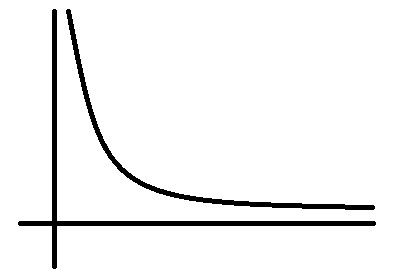
\includegraphics[width=8.3cm]{data/longtail}
  \end{center}
  \caption{The longtail: Items ordered by popularity are layed out against their popularity rating. Most of the items reside in the long tail of the graph.}
  \label{fig:longtail}
\end{figure}

Recommendation algorithms aim to filter out items within a data set that are of particular interest to the user, i.e. correspond to certain information within the user profile and/or its 'neighbourhood' \cite{burke2002}. In general, recommendation algorithms can be classified into one of three categories \cite{rajaraman2012}:

\begin{itemize}
	\item \textbf{Content-based filtering}: Using chosen or modelled features of items to define similarity between items in the user profile and candidate suggestions;
	\item \textbf{Collaborative filtering}: Using overlap of item sets of each user profile to find possible suggestions in the difference of these item sets;
	\item \textbf{Hybrid filtering}: Using a combination of content-based and collaborative approaches.
\end{itemize}

Each of these approaches has its strengths and weaknesses, but a common problem is that recommender systems appear to the end user as black boxes, generating item suggestions seemingly at random. Therefore, many applications have been developed to help provide transparancy into the recommendation process through a white box model. These explanation systems can then be used to make educated choices between item recommendations \cite{herlocker2000}.

In this paper we will look at the design and evaluation of an explanation system for collaborative filtering. First we will sketch the context of this paper looking from different angles. Next we will discuss the general idea and design of the explanation system, followed by an overview of the evaluation techniques and results. We conclude with a discussion of the results and some final conclusions.


\section*{RELATED WORK}

There are four major topics in this paper, namely: item recommendation, insight gaining processes, interactive visualization and graph drawing. As a result, each of these fields provides a different point of view on the subject of focus.


\subsection*{Recommender systems}

In a paper by Herlocker et al., a white box model for collaborative filtering is presented \cite{herlocker2000}. This paper has been an inspiration for other researchers to develop explanation systems. In \cite{o'donovan2008} an application called PeerChooser is presented by O'Donovan et al. It uses a graph-based visual explanation system of the collaborative filtering process that generates item suggestions. Also interactive elements are incorporated in the visualization to manipulate the active user's neighbourhood. The SmallWords application by Gretarsson et al. \cite{gretarsson2010} uses a similar approach. Pharos \cite{zhao2010} also builds on ideas brought forth in \cite{herlocker2000} and \cite{o'donovan2008}. The application computes a social map from the user's behaviour in content-based websites. The TasteWeights application by Bostandjiev et al. is created for a hybrid recommendation system. It uses a graph-based approach to visualize relationships between the different recommender algorithms \cite{bostandjiev2012}.

From the perspective of recommender systems, this research tries to apply concepts and techniques from insight gaining, sensemaking, interactive visualization and clutter reduction to design and implement a white box model for collaborative filtering.


\subsection*{Insight gaining}

In this paper, the main ideas on insight gaining are based on a literature study by Yi et al. \cite{yi2008}. In \cite{north2006}, Chris North discusses concepts related to insight, sensemaking and visualization presented in a paper \cite{klein2006} by Klein et al.

From the perspective of insight gaining and sensemaking, this paper tries to use the theory behind insight gaining and sensemaking, on visual explanation systems for collaborative recommendation. In this case the visualization provides the tool to support the insight gaining process. The process in which the user will try to gain insight, is item recommendation.


\subsection*{Interactive visualization}

Designing good visual explanation systems rely on techniques and principles of interactive visualization design. This includes taking into account physical limitations of the end user as described by Ware et al. \cite{ware2004}, as well as limitations in screen size and computational power, discussed by Shirley et al. and Ware et al. \cite{shirley2009, ware2004}. Various algorithms have been developed to reduce visual clutter in visualizations, avoiding visual overload. Ellis et al. have catalogued and categorized many of these algorithms in \cite{ellis2007}. Papers by Daniel Keim, Yi et al. and Chris North discuss the link between insight and visualization \cite{keim2002, yi2008, north2006}. In \cite{shirley2009}, \cite{ware2004} and \cite{keim2002}, an overview is given of visualization characteristics and principles, regarding data types, visual encodings, and data reduction and distortion techniques.

From the perspective of interactive visualization, this paper explores insight gaining through visualization, visualization as a means for discovery and visual datamining, and representative visual models for collaborative filtering.


\subsection*{Graph drawing}

This paper draws from ideas of a subfield of visualization, namely graph drawing. In \cite{herman2000} Herman et al. present an overview of graph drawing techniques. Techniques of the more general class of interactive visualization can be used to design and create graphs. In the domain of graph drawing, several specific clutter reduction algorithms, such as different types of clustering and edge-bundling \cite{herman2000, holten2009}, can be used as well. Another contribution to the field by Scott Murray, was to use alternative representations of connections between nodes of a graph, other than simple lines. It explores possibilities for encoding additional information in graphs in a transparant way \cite{murray2008}. Ware et al. look at three dimensional graph drawing as a solution to the problem of screen space limitations \cite{ware2008}.

This paper also uses ideas presented in a chapter by Valdis Krebs in \cite{steele2010}. Krebs applies dimensionality reduction on dual graphs to generate graphs based on just one set nodes of the dual case.

From a graph drawing perspective, this paper tries to illustrate the effectiveness of graph-based network visualization in the context of collaborative recommendation.



\section*{DESIGN}

\subsection*{Utility matrix}

The data used by the recommender system usually takes the form of a matrix in which users correspond to rows, and items correspond to columns. This matrix is often referred to as the utility matrix $M$. An entry $a_{i,j}$ in this matrix corresponds to a quantification of preference of user $i$ for item $j$. The goal of the recommendation algorithm is to find an estimation of the preference for blank entries in the matrix \cite{rajaraman2012}.

\begin{figure}[!ht]
  \begin{center}
  	% REMARK: To avoid bad boxes, use width 8.3cm or less. It is recommended
  	% to use .eps under dvips or .pdf under pdftex for good picture quality.
  	% You can convert eps to pdf using epstopdf.
  	
  	% EDIT: Replace mtits2011.pdf by your figure  	
    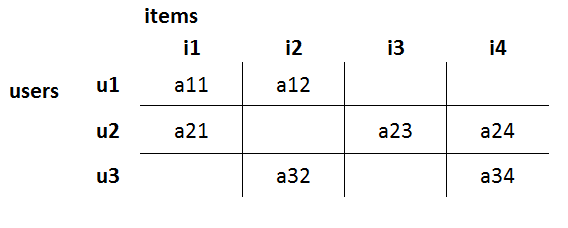
\includegraphics[width=8.3cm]{data/utility-matrix}
  \end{center}
  \caption{The utility matrix: the entries $a_{i,j}$ represent the degree of preference of a user $i$ for an item $j$.}
  \label{fig:utilitymatrix}
\end{figure}

Often the utility matrix is very sparse. For systems with thousands of users and items, users will generally only have rated a small subset of those items. The problem raises significant performance issues for new users, as they have few items in their rating history, or new items, as few people have that particular item in their rating history. This problem is often referred to as the cold start problem \cite{herlocker2000, rajaraman2012}.

Another issue that is typically related to collaborative filtering is the gray sheep problem. In this phenomenon, a user profile may have no or very few other similar users. This makes it hard to establish a true 'neighbourhood' for this user \cite{zhao2010}.


\subsection*{Conceptual model}

% http://www.proofwiki.org/wiki/Symbols:Set_Operations_and_Relations

In collaborative filtering relationships between users $u_{i} \in U$ are established through overlap between item sets $I_{i} \subseteq I$ contained in the user profiles, where $I$ represents the total item space. Items owned by one user that reside in the difference between these sets, are candidate item recommendations for the other user. This corresponds to non-blank entries within a column of the utility matrix.

If we define the set of items $I_{1}$ owned by user $u_{1}$ as $I_{1} \subseteq I$, a subset of the total set of items $I$, and the items $I_{2}$ owned by user two as $I_{2} \subseteq I$ and $I_{1} \cap I_{2} \neq \emptyset$. The candidate recommendation set $R_{1,2}$ is then defined as $I_{1} \setminus I_{2}$. In practice all the users $U$, or a significant subset of these users $U_{i} \subset U$, are taken into account when computing item recommendations.

From a graph-based point of view, relationships correspond to edges between nodes that correspond in turn to the users and items. In conclusion, the network is represented by a dual graph $G(V,E)$, for which $V = U \cup I$ such that $U \cap I = \emptyset \wedge E \subseteq U \times I$. An example of a dual graph is displayed in Figure \ref{fig:dualgraph}.

\begin{figure}[!ht]
  \begin{center}
  	% REMARK: To avoid bad boxes, use width 8.3cm or less. It is recommended
  	% to use .eps under dvips or .pdf under pdftex for good picture quality.
  	% You can convert eps to pdf using epstopdf.
  	
  	% EDIT: Replace mtits2011.pdf by your figure  	
    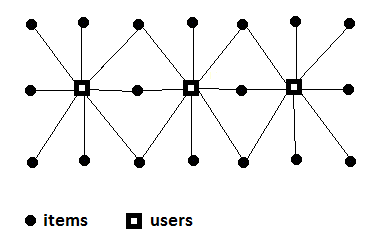
\includegraphics[width=8.3cm]{data/dual-graph}
  \end{center}
  \caption{Dual graph: There only exist edges that go from an item to a user or from a user to an item.}
  \label{fig:dualgraph}
\end{figure}

Due to sparsity in the utility matrix, the connectedness of the graph is likely to be very low. This becomes a problem for establishing a representative model, if there is little overlap between user profiles. This problem will manifest itself most prominently in the case of the cold start problem and the gray sheep problem, but even within a sample of the user's neighbourhood, results may be disappointing. A strategy to alleviate this problem may be to cluster neighbour profiles to a pseudo-neighbour to increase the chance of overlap.


\subsection*{Data and dimensionality reduction}

The example shown in Figure \ref{fig:dualgraph} is not representative of the graphs that would be generated from a utility matrix. In practice, many more nodes and edges bewteen them are involved, causing the typical scalability problems of graph drawing. When drawing medium to large-sized graphs, visual clutter is a main concern, and different approaches exist to solve the issue at least partially \cite{herman2000, holten2009, ellis2007, shirley2009, ware2004}.

Here we look at dimensionality reduction described in an example by Valdis Krebs in \cite{steele2010}. The idea is to obtain node reduction by combining pairs of edges originating from same user node to a single edge. The set of user nodes will then eventually be eliminated from the dual graph. If two users both share two items, this will result in two parallel edges between these item nodes. When applied over the whole graph, the strength of the relationship between pairs of items is then represented by the number of parallel edges between them. In \cite{steele2010}, Valdis Krebs went a step further and also clustered parallel edges. Strong connectedness can then be represented by edge thickness or brightness \cite{steele2010, shirley2009}. A simple example of this idea can be seen in Figure \ref{fig:dualgraph2}.

\begin{figure}[!ht]
  \begin{center}
  	% REMARK: To avoid bad boxes, use width 8.3cm or less. It is recommended
  	% to use .eps under dvips or .pdf under pdftex for good picture quality.
  	% You can convert eps to pdf using epstopdf.
  	
  	% EDIT: Replace mtits2011.pdf by your figure  	
    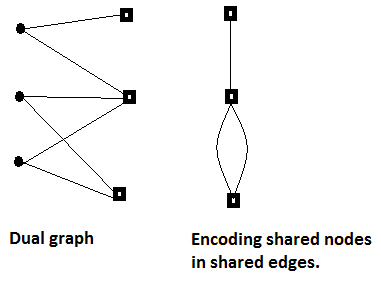
\includegraphics[width=8.3cm]{data/dual-graph2}
  \end{center}
  \caption{Eliminating one set of nodes in the dual graph by replacing shared nodes by shared edges.}
  \label{fig:dualgraph2}
\end{figure}

Although data fusion algorithms reduce information overload, they also introduce an important tradeoff in regard to insight gaining and sensemaking, as identified by Klein et al. Data transformation may pose challenges to sensemaking if the mental model of the system is inaccurate \cite{klein2006}. The quality of the visualization will therefore rely on the effectiveness of the user forming an accurate mental model \cite{herlocker2000, klein2006}.

In order to make estimates of the quality of each recommendation, it is important that certain contextual information does not get lost through dimensionality and data reduction techniques. The contextual information we want to convey is two-fold:

\begin{enumerate}
	\item The strength of the links between a recommendation and the user's profile;
	\item The position of the user in his/her neighbourhood and the relation with those neighbours.
\end{enumerate}

Since it may be unlikely that the whole user profile can be shown in the graph, the active user's favourite items are used to give a representation of the active user's profile. This way the user can still directly compare him/herself with neighbouring profiles.

To retain information about different users in the graph, we keep parallel edges. To deal with visual clutter introduced by a great number of edges, we apply an edge bundling technique described by Holten et al. in \cite{holten2009}. Edge bundling is a technique to let edges attract each other, making them follow a similar path. This techniques allows for faster pattern detection and reduces visual clutter \cite{holten2009}. Figure \ref{fig:edgebundling} shows a simple example how this concept is translated in a visualization.

\begin{figure}[!ht]
  \begin{center}
  	% REMARK: To avoid bad boxes, use width 8.3cm or less. It is recommended
  	% to use .eps under dvips or .pdf under pdftex for good picture quality.
  	% You can convert eps to pdf using epstopdf.
  	
  	% EDIT: Replace mtits2011.pdf by your figure  	
    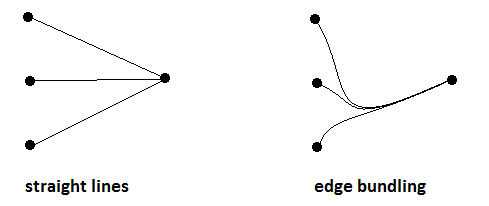
\includegraphics[width=8.3cm]{data/edge-bundling}
  \end{center}
  \caption{Edge bundling: edges are modelled as "flexible springs that can attract each other", similar to how electrical wires are bundled within a network \cite{holten2009}.}
  \label{fig:edgebundling}
\end{figure}


\section*{EVALUATION}

\subsection*{Research questions}

For the first evaluation of the prototype, the questions of focus were the following:

\begin{itemize}
	\item Does the user understand the conceptual model that the visualization is trying to convey?
	\item Does the conceptual help to identify reliable recommendations?
\end{itemize}


\subsection*{Paper prototype}

To test the effectiveness of the visualization, a paper prototype was constructed to use in user tests. The prototype consisted out of a default screen showing the initial state of the graph and a list of the users in the active user's neighbourhood. The active user's profile was highlighted on the graph.

The prototype was based on the utility matrix shown in Figure \ref{fig:matrixprototype}. The resulting visualization is shown in Figure \ref{fig:paperprototype1}. There is no guarantee that this prototype is scalable to an actual application. Analyzing a graph is easiest when a graph is small \cite{herman2000}, so we can assume that if this version is hard to understand, a version with many more items involved, will not perform any better.

Figures \ref{fig:paperprototype2} and \ref{fig:paperprototype3} show how the prototype would change if the test user would hover the icon of a neighbouring user profile and when the user hovers an item on the graph.

\begin{figure}[!ht]
  \begin{center}
  	% REMARK: To avoid bad boxes, use width 8.3cm or less. It is recommended
  	% to use .eps under dvips or .pdf under pdftex for good picture quality.
  	% You can convert eps to pdf using epstopdf.
  	
  	% EDIT: Replace mtits2011.pdf by your figure  	
    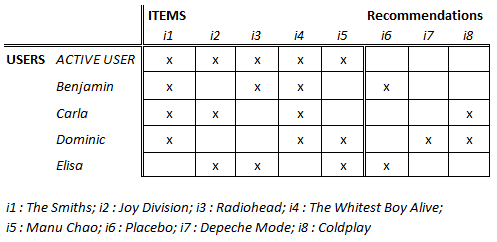
\includegraphics[width=8.3cm]{data/utility-matrix-prototype}
  \end{center}
  \caption{Utility matrix used in the paper prototype.}
  \label{fig:matrixprototype}
\end{figure}

\begin{figure}[!ht]
  \begin{center}
  	% REMARK: To avoid bad boxes, use width 8.3cm or less. It is recommended
  	% to use .eps under dvips or .pdf under pdftex for good picture quality.
  	% You can convert eps to pdf using epstopdf.
  	
  	% EDIT: Replace mtits2011.pdf by your figure  	
    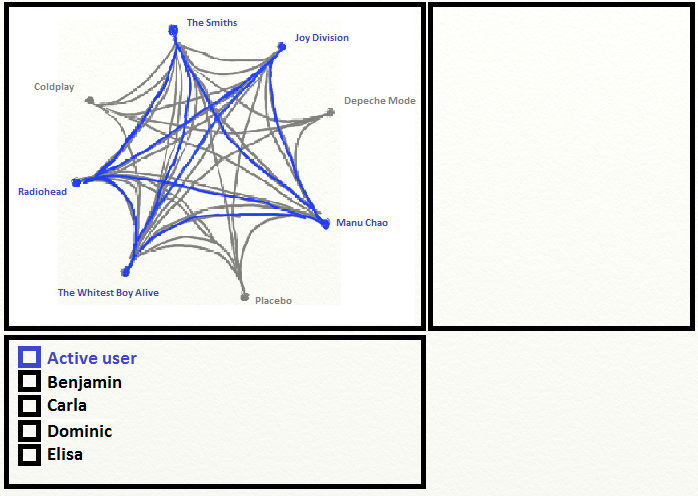
\includegraphics[width=8.3cm]{data/paperprototype1}
  \end{center}
  \caption{The default screen in the paper prototype.}
  \label{fig:paperprototype1}
\end{figure}

\begin{figure}[!ht]
  \begin{center}
  	% REMARK: To avoid bad boxes, use width 8.3cm or less. It is recommended
  	% to use .eps under dvips or .pdf under pdftex for good picture quality.
  	% You can convert eps to pdf using epstopdf.
  	
  	% EDIT: Replace mtits2011.pdf by your figure  	
    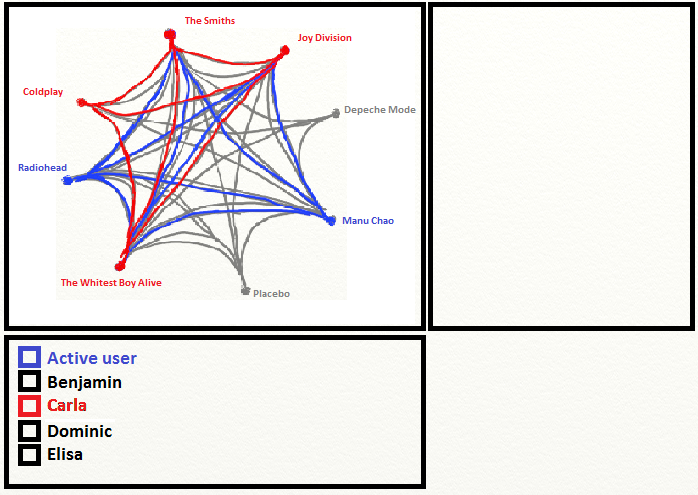
\includegraphics[width=8.3cm]{data/paperprototype2}
  \end{center}
  \caption{Highlighting a user profile, other than the active user's profile.}
  \label{fig:paperprototype2}
\end{figure}

\begin{figure}[!ht]
  \begin{center}
  	% REMARK: To avoid bad boxes, use width 8.3cm or less. It is recommended
  	% to use .eps under dvips or .pdf under pdftex for good picture quality.
  	% You can convert eps to pdf using epstopdf.
  	
  	% EDIT: Replace mtits2011.pdf by your figure  	
    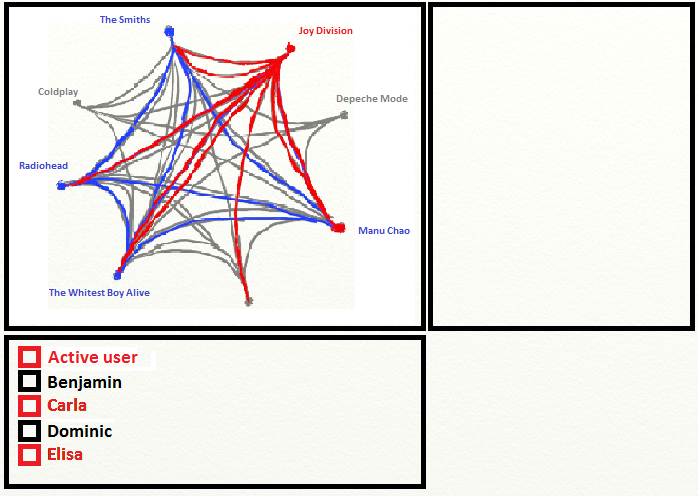
\includegraphics[width=8.3cm]{data/paperprototype3}
  \end{center}
  \caption{Highlighting an item in the graph.}
  \label{fig:paperprototype3}
\end{figure}


\subsection*{Method}

Five test users, male and female, were selected within the age-group of 22 to 25. The test started by providing some context in which the system could be used. They performed a series of tasks using the paper prototype while applying the think aloud protocol. At the end of the test, the user filled in a system usability scale questionnaire. The following tasks were executed by the test users:

\begin{enumerate}
	\item Study the visualization without interacting with it. Describe what you see. Describe what you expect the visualization does.
	\item Interact with the visualization by clicking and hovering visual elements. Explain which items are suggestions. Explain who the other users are. Explain which information is contained in a link between two items.
	\item Add a suggestion to your profile. Give one or more reasons why this would be a reliable suggestion.
\end{enumerate}

The first part of the test, corresponding to tasks one and two, was to see how the user would go about establishing the mental model of the system. This set of tasks was based on the insight gaining process described by Yi et al. in \cite{yi2008}. This is an iterative process consisting of four stages that are intertwined and self-generating \cite{yi2008}:

\begin{itemize}
	\item \textbf{Provide overview}: in this process the individual gains understanding of the big picture of a dataset of interest. It allows the user to make a distinction between what is known to him/her and what is not;
	\item \textbf{Adjust}: in this process a person will explore a dataset by adjusting the level of abstraction and/or the range of selection. Typical actions involve filtering and grouping of data;
	\item	\textbf{Detect pattern}: in this process the user will try to identify specific distributions, trends, frequencies, outliers or structure in the dataset;
	\item \textbf{Match mental model}: in this process the gap between data and cognitive model is bridged, reducing cognitive load and linking the present visual information with real-world knowledge;
\end{itemize}

In the third task of the test, the user had to try out the main functionality of the system, i.e. adding a suggestion to his/her profile. The goal of this task is two-fold:

\begin{itemize}
	\item establishing to what extend th conceptual model was understood;
	\item verifying if the application was easy to use once the conceptual model was understood.
\end{itemize}


\subsection*{Results}

During task one, almost all of the users interpreted the links between the artists in the visualization as a content-based relationship, e.g. genre. One user interpreted the links correctly. The reason was that this user connected the highlighted items to the highlighted user. In a second step, the edges of the graph were correctly identified as a co-occurance relationship. Interestingly this is usually how the other test users would adjust their wrong conceptual model in during the second step. For the user that had the model correct in step one, the second task was merely a confirmation of this model.

As mentioned earlier, the second task usually corresponded to adjusting the mental model of the system. All the test users managed to get the conceptual model right at the end of the second task. However, some of these users were given a little hint what to look for. As a result there was a consensus that given some textual help, the learnability of the system would improve significantly.

Task three turned out to be a formality for most of the test users. All of the test users could give an adequate reason for chosing a particular suggestion, e.g. many users that have the suggested item in their profile.

The average overall score on the SUS questionnaire for the five participants was $77.0$ out of a maximum of $100.0$.


\section*{FINAL THOUGHTS}

In this paper we have looked at a new white box model for collaborative filtering using a graph-based visualization as a solution to the black box problem. This model tries to apply dimensionality reduction techniques in combination with edge bundling to reduce visual clutter and visual overload. We have tried to evaluate this model through a paper prototype and using think aloud protocol and tasks based on the insight gaining process.

Overall the results are promising, but far from perfect. There are still other research questions that could be answered; for example how does the application perform in alleviating the cold start problem. Also additional functionality can be included. Some of the test users suggested to include a possibility to select items from their library to use in the visualization.

Future work includes testing improved prototype and the implementation and evaluation of the model in an application.


%\bibliographystyle{nar}
\bibliographystyle{abbrv}
\bibliography{data/references}	% EDIT: Replace 'mtits2011' by your BibTeX database file

\end{document}
